\documentclass{amsart}
\usepackage{amssymb}
\usepackage{amsaddr}
\usepackage[utf8]{inputenc}
%\usepackage[T1]{fontenc}
\usepackage[english]{babel}
\usepackage{csquotes}
\usepackage{comment}
\usepackage{xargs}
\usepackage{graphicx, color}
\setkeys{Gin}{draft=false}
\usepackage[figurewithin=none]{caption,subcaption} 
\graphicspath{{./img/}} %Uso: \graphicspath{{RelativePath}}
% \newcommand{\src}{./source}
\usepackage{enumitem}
\setlist[enumerate,1]{label={(\roman*)}}

\usepackage[sfdefault]{arimo}
\usepackage[T1]{fontenc}


%% Linenumbers
\usepackage[pagewise,modulo,mathlines]{lineno}
\linenumbers
\renewcommand{\linenumberfont}{\normalfont\bfseries\scriptsize\color{cyan}}

\usepackage[notcite,notref,color,]{showkeys}

 \usepackage{hyperref}
 \hypersetup{
 	hidelinks,
   colorlinks  = true,    % Colours links instead of ugly boxes
   urlcolor    = blue,    % Colour for external hyperlinks
   linkcolor   = blue,    % Colour of internal links
   citecolor   = blue,      % Colour of citations
   pdfauthor   = {Javier Bracjo, Daniel Gonzáles-Casanova, Isabel Hubard, Elías Mochán, Antonio Montero },%
   pdfsubject  = {Chiral},%
   pdftitle    = {Two new chiral 4-polytopes in $\mathbb{E}^4$},  
}
\usepackage{float}
\usepackage[capitalise,noabbrev, nameinlink,]{cleveref}
\usepackage{tikz-cd}
\tikzcdset{%
row sep=tiny,%
arrows={shorten=-4pt}
% start anchor = center, %
% end anchor = center%
}

\usepackage[loadshadowlibrary,shadow, colorinlistoftodos,textsize=tiny,obeyFinal]{todonotes}

%if you need to use a twosided document but you want the to-dos on the right (left) margin, uncomment the following lines.
% \makeatletter 
% \@mparswitchfalse%
% \makeatother
% \normalmarginpar %for right-handed notes and lines, or 
% %\reversemarginpar %if you want them on the left of your twosided document. 

\setuptodonotes{fancyline, backgroundcolor=gray!10,bordercolor=gray}
\newcommand{\missingref}[1][?]{\todo[color=gray!30]{Reference (#1)}}



%%Other examples of todonotes %requires xargs
\newcommandx{\inline}[2][1=]{\todo[inline, #1]{#2}}
\newcounter{hw}
\setcounter{hw}{1}
\newcommandx{\homework}[2][1=]{\todo[inline, caption={Homework \thehw} #1]{\stepcounter{hw} #2}}

%
 \newcommand{\isa}[1]{\todo[color=green!25]{\textbf{Isa:}#1}}
 \newcommand{\elias}[1]{\todo[color=red!25]{\textbf{Elías:} #1}}
 \newcommand{\tero}[1]{\todo[color=blue!25]{\textbf{Tero:} #1}}

 \newcommandx{\isaLong}[2][1=Long todo, usedefault]{\todo[inline, color=green!25, caption={\textbf{Isa:} #1}]{\textbf{Isa: #1}. #2}}
 \newcommandx{\eliasLong}[2][1=Long todo, usedefault]{\todo[inline, color=red!25,caption={\textbf{Roli:} #1}]{\textbf{Elías: #1}. #2}}
 \newcommandx{\teroLong}[2][1=Long todo, usedefault]{\todo[inline,color=blue!25, caption={\textbf{Dani:} #1}]{\textbf{Tero: #1}. #2} }

\makeatletter
    \providecommand\@dotsep{5}
\makeatother

%[problem]

\input{source/authorThm}


\input{source/authorCmd}


\usepackage[%
sorting=nyt, %
backend=biber, %
style=numeric,%
defernumbers=true,%
% sorting=ydnt,%
url=false,%
eprint=false,%
giveninits=true,
maxbibnames=9,%
% doi=false,%
isbn=false,%
sortcites = true,%
citestyle=numeric-comp,
]{biblatex}
\addbibresource{biblio.bib}






\begin{document}

\title{Two new chiral 4-polytopes of full rank}
\author{Javier Bracho} 
\address{Institute of Mathematics, National Autonomous University of Mexico (IM UNAM), 04510 Mexico City, Mexico}
\email{jbracho@im.unam.mx}
\author{Daniel Gonz\'alez-Casanova}
\address{Institute of Mathematics, National Autonomous University of Mexico (IM UNAM), 04510 Mexico City, Mexico}
\email{dag@ciencias.unam.mx}
\author{Isabel Hubard}
\address{Institute of Mathematics, National Autonomous University of Mexico (IM UNAM), 04510 Mexico City, Mexico}
\email{isahubard@im.unam.mx}


\begin{abstract}
In the setting of skeletal geometric complexes, chiral polytopes are those possessing maximal rotational symmetry while lacking reflection symmetry. We demonstrate that the natural rotation about the base edge in two chiral polyhedra from \cite{petcox} generates, in each case, a chiral 4-polytope in $\E^4$. Furthermore, both resulting polytopes are shown to be combinatorially chiral. 

\end{abstract}

\maketitle 

% \tableofcontexnts

\listoftodos\relax

\section{Introduction}

The study of polygons and polyhedra dates back to antiquity, yet their precise definitions have evolved significantly over time. Early mathematical texts, such as Euclid’s Elements, focused on regular convex polygons and the five Platonic solids, establishing a foundation that persisted for centuries. Over time, mathematicians extended these ideas to more general structures, including non-convex and higher-dimensional polytopes.

A key shift in perspective occurred in the 20th century with the introduction of the skeletal approach, in which polygons are considered as 1-dimensional complexes, and polyhedra are built from them, rather than requiring enclosed surfaces or solids.
This approach enables the study of new symmetry types, including {\em chiral polytopes}, that exhibit maximal rotational symmetry but lack reflection symmetry. 
%In contrast to regular polyhedra, whose symmetry groups act transitively on the set of flags (incident vertex-edge-face triples), a polyhedron is said to be geometrically chiral when its symmetry group has two orbits on the flags, with so-called adjacent flags belonging to distinct orbits.

Chiral polyhedra in ordinary space were first  classified in 2005, when Schulte identified those realizable in Euclidean 3-space, none of which are finite or have planar faces \cite{chiral-polyhedra-i,chiral-polyhedra-ii}. Nearly a decade later, the first example of a chiral 4-polytope in $\E^4$, was constructed by Bracho, Hubard, and Pellicer \cite{rolis-cube}. 
Subsequent work revealed that the facets of this polytope belong to a broader family of chiral polyhedra with helical faces in $\mathbb{S}^3$ \cite{petcox}.


This paper builds upon these developments by constructing new examples of chiral 4-polytopes in $\mathbb{E}^4$. 
Specifically, we show that a natural rotation about the base edge in two previously studied spherical polyhedra successfully produces, in each case, a chiral 4-polytope. 
Moreover, we establish that their combinatorial structures are also chiral, a property not shared by their facets, which remain combinatorially regular.

To verify these results, we employ computational methods using GAP programs, allowing us to compare the abstract and geometric structures rigorously. The geometric realizations rely on reflection matrices introduced in \cite{petcox}.%, and all computational tools developed for this study are available online (see \Cref{app:A}).

By exploring the interplay between geometry, symmetry, and combinatorial structure, this work contributes to the broader understanding of chiral polytopes and their role in polytope theory. 
The results presented here not only extend previous classifications but also open new avenues for the study of chirality in higher-dimensional spaces.


	
	\section{Skeletal polyhedra and 4-polytopes in $\E^4$}\label{sec:skeletal}
	%Now we give formal definitions and basic results.
	
	A \textit{skeletal polyhedron} in $\E^4$ consists of \textit{vertices} (points in $\E^4$), \textit{edges} (segments between vertices) and \textit{faces} (cycles on the graph determined by the vertices and edges) such that:
    
	\begin{enumerate}%[\itshape(i)]
		\item every edge belongs to two faces,
		\item the graph determined by the vertices and edges is connected,
		\item every compact subset of $\E^4$ meets finitely many edges, and
		\item the \textit{vertex-figure}, defined as follows, is a connected graph. For any vertex $v$, the vertices of the vertex-figure are the neighbours of $v$ and the edges are segments joining any two neighbours that are both in some face.
	\end{enumerate}
    
	A \textit{skeletal 4-polytope} in $\E^4$ consits of vertices, edges, faces and \textit{cells} (skeletal polyhedra), such that
    
	\begin{enumerate}%[\itshape(i)]
		\item every face belongs to two cells,
		\item the graph determined by the vertices and the edges is connected,
		\item every compact subset of $\E^4$ meets finitely many edges, and
		\item the vertex-figure at every vertex is a skeletal polyhedron.
		\end{enumerate}
	
	Hereafter we omit the term "skeletal" when the context permits it. If $\p$ is a 4-polytope, the set of vertices, edges, faces and cells is a partial order with respect to inclusion. We say two such elements are \textit{incident} if they are comparable. This poset is called the \textit{abstract polytope associated to $\p$}. As we shall see, 4-polytopes defined as above are realizations of abstract polytopes in the sense of \cite{ARP} and \Cref{sec:abstract-defs}.
	
	A \textit{flag} is a 4-tuple of incident vertex, edge, face and cell. Two flags are \textit{adjacent} when they differ by only one element. We call two flags \textit{0-adjacent} if they differ by a vertex, \textit{1-adjacent} if they differ by an edge, \textit{2-adjacent} if they differ by a face and \textit{3-adjacent} if they differ by a cell.
	
	A \textit{symmetry} of $\p$ is an isometry of $\E^4$ that preserves it set-wise. The group of symmetries of $\p$ will be denoted by $G(\p)$. We call $\p$ \textit{regular} if $G(\p)$ acts transitively on the set of flags, and \textit{chiral} if $G(\p)$ induces two orbits on flags so that adjacent flags are on different orbits. In fact, whether $\p$ is regular or chiral, its symmetry group acts transitively on the sets of vertices, edges, faces and cells.
	

	
\section{Abstract 4-polytopes}\label{sec:abstract-defs}
	The theory of abstract polytopes is an essential tool for our work. In this section we state basic results and constructions upon which our proofs are based. To avoid using the word 'abstract' in every definition, we use the same words as in the previous section to mean different objects. All polytopes are abstract up to \Cref{subsec:realizations}, where they are precisely distinguished.
	
	An \textit{abstract $4$-polytope} is a partial order $\p$ that satisfies the following properties (P1) to (P4). The elements of $\p$ are called \textit{faces} and the maximally ordered subsets (chains) are called \textit{flags}.
	\begin{enumerate}
		\item[(P1)]\label{P1} $\p$ contains a minimal face and a greatest face, denoted respectively by $F_{-1}$ and $F_4$.
		\item[(P2)]\label{P2} Flags contain $6$ elements, including $F_{-1}$ and $F_4$.
	\end{enumerate}
	Since every element in a poset is in some chain, we may assign to every face a number from $-1$ to $4$. Such is the \textit{rank function} of $\p$. We say that two flags are \textit{$i$-adjacent} if they differ only by a face of rank $i$.
	\begin{enumerate}
		\item[(P3)]\label{P3} $\p$ is \textit{strongly flag connected} in the following sense. For any two distinct flags $\Phi$ and $\Psi$ there is a sequence
		\[\Phi=\Phi_0,\Phi_1,\ldots,\Phi_k=\Psi\]
		so that $\Phi_{i-1}$ and $\Phi_i$ are adjacent and $\Phi\cap\Psi\subset\Phi_i$ for all $i$.
		\item[(P4)]\label{P4} If $F$ and $G$ are a $(i-1)$-face and a $(i+1)$-face with $F<G$ and $0\leq j\leq2$, then there are exactly two $i$-faces $H$ such that $F<H<G$.
	\end{enumerate}
	
		\subsection{Regular and chiral abstract 4-polytopes}
	Now we study regular 4-polytopes and their automorphism groups. An \textit{automorphism} of $\p$ is a bijection of the polytope that preserves incidence, and we denote the automorphism group by $\Gamma(\p)$. $\p$ is called \textit{regular} if $\Gamma(\p)$ is transitive on flags.
	
	For a regular polytope $\p$ and some distinguished flag $\Phi$, there exists a unique involutory automorphism $\rho_j$ of $\p$ such that $\Phi\rho_i=\Phi^i$ for $i=0,1,2,3$ (Prop. 2B4, \cite{ARP}). These are called the \textit{distinguished generators} of $\Gamma(\p)$ and satisfy that 
	\begin{equation}\label{eq:string-reg}
			(\rho_i\rho_j)^{p_{ij}}=\Id\text{ when } |i-j|\geq2\
	\end{equation}
	for $i,j=0,1,2,3$ (prop. 2B11 \cite{ARP}). The numbers $p_i:=p_{i-1}p_i$ form the \textit{Schläfli type} $\{p_1,p_2,p_3\}$ of $\p$. The distinguished generators also satisfy 
	\begin{equation}\label{eq:int-reg}
		\langle \rho_i|i\in I\rangle\cap\langle\rho_j|j\in J\rangle=\langle\rho_i\in I\cap J\rangle\qquad\text{for }I,J\subseteq\{0,1,2,3\}
	\end{equation}
	which we call the \textit{intersection property} (prop. 2B10 \cite{ARP}). Any group $\Gamma$ generated by the involutions $\rho_0$ to $\rho_3$ satisfying \cref{eq:string-reg,eq:int-reg} is called a \textit{C-string group}. We have established that $\Gamma(\p)$ is one such group.
	
	Conversely, we may construct a regular abstract $4$-polytope from a C-string group $\Gamma$. Define $\Gamma_j:=\langle\rho_j|i\neq j\rangle$ and $\Gamma_{-1}=\Gamma_4=\Gamma$, and take the set of $i$-faces to be the set of right cosets $\Gamma_i\varphi$ for $\varphi\in\Gamma$. Then there is an order relation with respect to which the set of all faces is a regular $4$-polytope whose automorphism group is $\Gamma$ (thm. 2E11, \cite{ARP}).
	
	\vspace{.5cm}
	
	Now we revise the analogue construction for chiral polytopes. An abstract 4-polytope $\p$ is called \textit{chiral} if $\Gamma(\p)$ induces two orbits on flags and two adjacent flags are in different orbits.
	
	First observe that by defining $\sigma_i:=\rho_{i-1}\rho_i$ for the distinguished generators of a regular polytope with bipartite flags, it holds that
	\begin{equation}\label{eq:chiral-rels}
		\begin{aligned}
			\sigma_1^{p_1}=\sigma_2^{p_2}&=\sigma_3^{p_3}=\Id\\
			(\sigma_1\sigma_2)^2=(\sigma_1\sigma_2&\sigma_3)^2=(\sigma_2\sigma_3)^2=\Id
		\end{aligned}
	\end{equation}
	for some positive integers $p_1$, $p_2$ and $p_3$ (see \cite{egon-asia-chiral}).
	
	The group generated by these elements is called the \textit{rotation subgroup} of $\p$, denoted by $\Gamma^+(\p)$. For chiral polytopes this will be the whole group: if $\p$ is chiral, $\Gamma(\p)$ is generated by three automorphisms $\sigma_1,\sigma_2$ and $\sigma_3$ that satisfy \cref{eq:chiral-rels} (prop. 3, \cite{egon-asia-chiral}).
	
	To construct a chiral or regular abstract polytope from a group we must also require some sort of intersection property. It will suffice that
	\begin{equation}\label{eq:chiral-int}
		\begin{aligned}
			\langle\sigma_1\rangle\cap\langle\sigma_2\rangle=\{\Id\}&=\langle\sigma_2\rangle\cap\langle\sigma_3\rangle\\
			\langle\sigma_1,\sigma_2\rangle\cap\langle\sigma_2,&\sigma_3\rangle=\langle\sigma_2\rangle.
		\end{aligned}
	\end{equation}
	Let $\Gamma=\langle \sigma_1,\sigma_2,\sigma_3\rangle$ be a group satisfying both \cref{eq:chiral-rels,eq:chiral-int}. Define
	\begin{align*}
		\Gamma^0=\langle\sigma_2,\sigma_3\rangle,\quad
		\Gamma^1=\langle \sigma_3,\sigma_1\sigma_2\rangle,\quad
		\Gamma^2=\langle &\sigma_1,\sigma_2\sigma_3\rangle,\quad
		\Gamma^3=\langle \sigma_1,\sigma_2\rangle,\\
		\text{and}\quad\Gamma_{-1}=\Gamma^4=\Gamma,
	\end{align*}
	and take the $i$-faces to be the right cosets $\Gamma_i\varphi$ for $\varphi\in\Gamma$. Again, the set of all faces admits a partial order with respect to which it is a chiral or a regular abstract 4-polytope $\p$ such that $\Gamma^+(\p)=\Gamma$ (thm. 1 and lem. 11, \cite{egon-asia-chiral}).
	
	In this construction we may distinguish chiral from regular abstract 4-polytopes as follows. $\Gamma^+(\p)$ is of index 2 in $\Gamma(\p)$ if and only if there exists an involutory automorphism $\rho:\Gamma\to \Gamma$ such that
	\begin{equation}\label{eq:combinatorially-chiral}
		\rho(\sigma_1)=\sigma_1^{-1},\quad \rho(\sigma_2)=\sigma_1^2\sigma_2\quad\text{and}\quad \rho(\sigma_3)=\sigma_3,
\end{equation}
	in which case $\p$ cannot be chiral (thm. 1, \cite{egon-asia-chiral}).

\vspace{10pt}

	\subsection{Realizations}\label{subsec:realizations}
	Now we review the relationship between abstract and skeletal polytopes as defined in \Cref{sec:skeletal}.
	
	A \textit{realization} of an abstract polytope $\p$ is a map $\beta$ from the set of abstract 0-faces $\p_0$ into $\E^4$, so that the set $V_0:=\p_0\beta$ is the set of geometric vertices. All other geometric faces are defined by functions from the set of abstract $i$-faces $\p_i$ to some nested power set of the geometric vertex set: edges are sets of vertices, faces are sets of edges and so on.
	
	Formally, for $i=1,2,3$, $\beta$ induces a surjection $\beta_i:\p_i\to V_i$, where $V_i$ is thought as the set of geometric $i$-faces, consisting of the elements ${F\beta_i:=\{G\beta_{i-1}|G\in\p_{i-1}\text{ and }G\leq F\}}$ for $F\in\p_i$ (thm. 5A1, \cite{ARP}). For example, an abstract edge $E\in\p_1$ is mapped to a set consisting of the two points (there's only two by (P4)) in $\E^4$ whose preimages are abstract vertices smaller than $E$ in $\p$.

	
%	Let the set of $i$-faces of an abstract polytope $\p$ be denoted by $\p_i$. Define $V_0:=\p_0\beta$ and $V_j$ to be the set consisting of elements of the form $F\beta_j:=\{G\beta_{j-1}|G\in\p_{j-1}\text{ and }G\leq F\}$ for $F\in\p_j$ and any $j$. Then $\beta$ induces surjections $\beta_j:\p_j\to V_j$. A realization is \textit{faithful} when each $\beta_j$ is a bijection.

	Of course, we expect the number of $i$-faces of the abstract and geometric structures to be the same. A realization is \textit{faithful} if every $\beta_i$ is a bijection.
	
	We also expect automorphisms to correspond with isometries of $\E^4$. A realization is \textit{symmetric} when every automorphism of $\p$ induces a permutation of $V_0$, which in turn determines a unique isometry of $\E^4$ (if the vertex set affinely spans $\E^4$). Then these isometries are an euclidean representation of $\Gamma(\p)$.
	
	Conversely, given an euclidean representation of the automorphism group $\Gamma(\p)$ of an abstract 4-polytope, we obtain a realization by \textit{Wythoff's construction} as follows.
	
	For the regular case, let $\langle R_0, R_1,R_2,R_3\rangle$ be an euclidean representation of the automorphism group of a regular abstract 4-polytope $\p$. Should there be any, define a point $v\in\E^4$ that is fixed by $R_1$, $R_2$ and $R_3$ but not by $R_0$ as the base vertex and take the orbit of $v$ for the geometric vertex-set of a realization. Further, define the base edge $e=v\langle R_0\rangle$, the base face $f=e\langle R_0,R_1\rangle$ and the base cell $c=f\langle R_0,R_1,R_2\rangle$ for a geometric base flag.
	
	Now let $\langle S_1,S_2,S_3\rangle$ be a representation of the automorphism group, or rotation subgroup, of a chiral or regular abstract 4-polytope, respectively. For a geometric base vertex choose any point that is fixed by $S_2$ and $S_3$ but not by $S_1$. The orbit of this point is the geometric vertex-set of a realization. For a geometric flag we define the base edge as $e=v\langle S_1S_2\rangle$, or equivalently, as $e=\{v,vS_1^{-1}\}$ since $S_1^{-1}=R_1R_0$ when $\p$ is regular. Define the base face as $f=e\langle S_1\rangle$ and the base cell as $c=f\langle S_1,S_2\rangle$.
	
	It is straightforward to check that a regular or chiral skeletal 4-polytope as defined in \Cref{sec:skeletal} is a faithful and symmetric realization of the abstract 4-polytope related to it.
	
	\vspace{.5cm}
	
	It remains only to formally define star polytopes. Following Section 7D from \cite{ARP}, we say a faithfully realized abstract 4-polytope is \textit{classical} if every geometric $i$-face has dimension $i$ (its affine hull is $i$-dimensional). For any such geometric regular polytope, we may write its generating hyperplane reflections as
	\[R_i=\{x\in\E^4|\langle x,u_i\rangle=0\}\]
	for some unit vectors $u_i$. Then $\langle u_i,u_j\rangle=0$ for $|i-j|\geq2$, and, since $\langle R_i,R_j\rangle$ is a finite group, there is a rational number $p_i$ such that $\langle u_{i-1},u_i\rangle=\cos(\pi/p_i)$. We define the \textit{Shläfli type} of this polytope as $\{p_1,p_2,p_3\}$ and call it a \textit{star 4-polytope} if any of the $p_i$ is not an integer. Of course, the definition for polyhedra is analogous.

	\section{A realization of $\left\{\frac{5}{2},3,5\right\}$}
	Our first chiral polytope will have the same vertices and edges as the star 4-polytope $\left\{\frac{5}{2},3,5\right\}$. We shall start by constructing $\left\{\frac{5}{2},3,5\right\}$ from a given realization of $\{3,3,5\}$. To this end we first express the generating reflections of $\left\{\frac{5}{2},3,5\right\}$ in terms of those of $\{3,3,5\}$. Then we prove they generate a C-string group, which in turn yields an abstract polytope. Finally we show it is realized as $\left\{\frac{5}{2},3,5\right\}$.
	
	Our construction is based in the following observations. In the regular star polyhedron $\left\{\frac{5}{2},3\right\}$ the edges intersect at points that are not vertices, and the convex hull of these intersections is a regular icosahedron. The vertex-figure of $\{3,3,5\}$ is also a regular icosahedron. Further, the vertices of $\left\{\frac{5}{2},3,5\right\}$ must be the same as those of $\{3,3,5\}$ (\cite{ARP}, p. 212).
	
	We are thus inclined to look for a copy of $\left\{\frac{5}{2},3\right\}$ within $\{3,3,5\}$ by taking the vertex-figure icosahedron of some vertex and at each of its faces consider the ajacent tetrahedron that is not contained in the interior of the icosahedron. We may visualize this by stereographically projecting the vertices and taking the convex hull of each tetrahedron as in \cref{fig:fig1}.
    
	\begin{figure}[h]
	\centering
	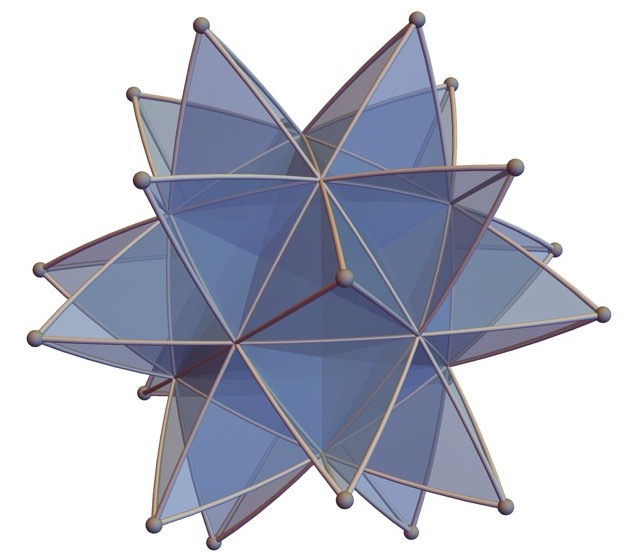
\includegraphics[width=0.4\linewidth]{FacetaPadrino.jpg}
	\caption{The base cell of $\left\{\frac{5}{2},3,5\right\}$ projected to the 3-sphere $\mathbb{S}^3$ and then to $\mathbb{R}^3$ by stereographic projection from the antipode of its centroid which is a vertex of $\left\{3,3,5\right\}$.}
	\label{fig:fig1}
	\end{figure}
	
	Notice that an edge of $\left\{\frac{5}{2},3\right\}$ is composed of three edges of $\{3,3,5\}$. Choosing a geometric flag for $\left\{\frac{5}{2},3,5\right\}$ amount to selecting an incident vertex, edge and face within this figure, which is the base cell.  We define the generating reflections of the symmetry group of $\left\{\frac{5}{2},3,5\right\}$ with respect to the base flag as follows. Call the base vertex $w_0$, the centroid of the base edge  $w_1$, the centroid of the base face  $w_2$ and the centroid of the base cell  $w_3$. The mirror of the reflection $P_i$ is the hyperplane through the origin and the $w_j$ such that $j\neq i$.
	
	There is a choice of base flag for $\{3,3,5\}$ for which the generating reflections $R_0$ to $R_3$ satisfy the following relations, that we shall use as definitions:
	\begin{gather*}
		P_0=R_0,\qquad P_2=R_3,\qquad P_3=R_2\\
		P_1=R_1R_2R_3R_2R_1R_0R_1R_2R_3R_2R_1
	\end{gather*}
	To construct a realization of $\left\{\frac{5}{2},3,5\right\}$ we first suppose that $R_0$ to $R_3$ are the distinguished generators of the abstract polytope $\{3,3,5\}$. That is, they satisfy the relations
	\[R_i^2=(R_0R_1)^3=(R_1R_2)^3=(R_2R_3)^5=(R_0R_2)^2=(R_0R_3)^2=(R_1R_3)^2=\Id\]
	for all $i$ and the intersection property. It has been confirmed that
		\[P_i^2=(P_0P_1)^5=(P_1P_2)^3=(P_2P_3)^5=(P_0P_2)^2=(P_0P_3)^2=(P_1P_3)^2=\Id\]
	for all $i$, and that the intersection property holds (see \Cref{app:1}). Then the abstract polytope generated by $P_0$ to $P_3$ is $\{5,3,5\}$.
	
	Using a particular realization of $\{3,3,5\}$, we may explicitly find the base vertex for $\left\{\frac{5}{2},3,5\right\}$ (see \Cref{app:coords}). Then Wythoff's construction yields a realization that we expect to be faithful and symmetric. Faithfullness follows by comparing the number of $i$-faces of the abstract polytope and the realization (see \Cref{app:1,app:2}). Symmetry follows from the fact the vertex-set of both $\{3,3,5\}$ and $\left\{\frac{5}{2},3,5\right\}$ is the same.
	
	Since the $R_i$ are hyperplane reflections, we have a classical polytope as defined in \Cref{subsec:realizations} (see \cite{mcmullen-4dimensional}). The only such polytopes in $\mathbb{E}^4$ arising from the abstract regular polytope $\{5,3,5\}$ are the star 4-polytopes $\left\{\frac{5}{2},3,5\right\}$ and $\left\{5,3,\frac{5}{2}\right\}$ (thm. 7D13 \cite{ARP}). However, the rotation about the edge in this polytope is the reverse of that of $\{3,3,5\}$, so that it cannot be of type $\frac{5}{2}$. This completes the proof that we have constructed $\left\{\frac{5}{2},3,5\right\}$.
	
	\section{A chiral 4-polytope from $\left\{\frac{5}{2},3,5\right\}$}
	To construct a chiral 4-polytope within $\left\{\frac{5}{2},3,5\right\}$, let
		\[S_1=P_0P_1P_3P_2,\qquad S_2=P_2P_1,\quad\text{and}\quad S_3=P_3P_2.\]
	Then
	\begin{equation}\label{eq:string-chiral}
		S_1^{12}=S_2^3=S_3^5=(S_1S_2)^2=(S_1S_2S_3)^2=(S_2S_3)^2=\Id
	\end{equation}
	and \cref{eq:chiral-int} holds (see \Cref{app:1}). It follows that the group generated by $S_1$ to $S_3$ yields either a regular or a chiral abstract polytope.
	
	For a realization by Wythoff's construction define the base vertex to be the same as the one that was used for $\left\{\frac{5}{2},3,5\right\}$. Such a choice and the fact that the group $\langle S_1,S_2,S_3\rangle$ a subgroup of $\langle P_0,P_1,P_2,P_3\rangle$ make the realization symmetric. Again, by comparing the number of $i$-faces in the abstract and geometric polytopes, our realization is seen to be faithful.
	
	The definitions of $S_1$ and $S_2$ are as in  \cite{petcox}, so that the cells are copies of the chiral polyhedron denoted as $H_1(\left\{5,3,\frac{5}{2}\right\})$. In fact, chirality in our 4-polytope follows from the chirality of the cells, since any symmetry sending a flag to its $i$-th adjacent is also a symmetry of the cell.
	
	We have shown this structure to have 120 vertices, 720 edges, 300 faces and 50 cells. Every face has 12 vertices and edges arranged in helical fashion as shown in \cite{petcox} (see \cref{fig:12}). In virtue of such arrangement we denote this polytope by $\left\{\frac{12}{1,5},3,5\right\}$.

\begin{figure}[H]
	\begin{center}
			\centering
			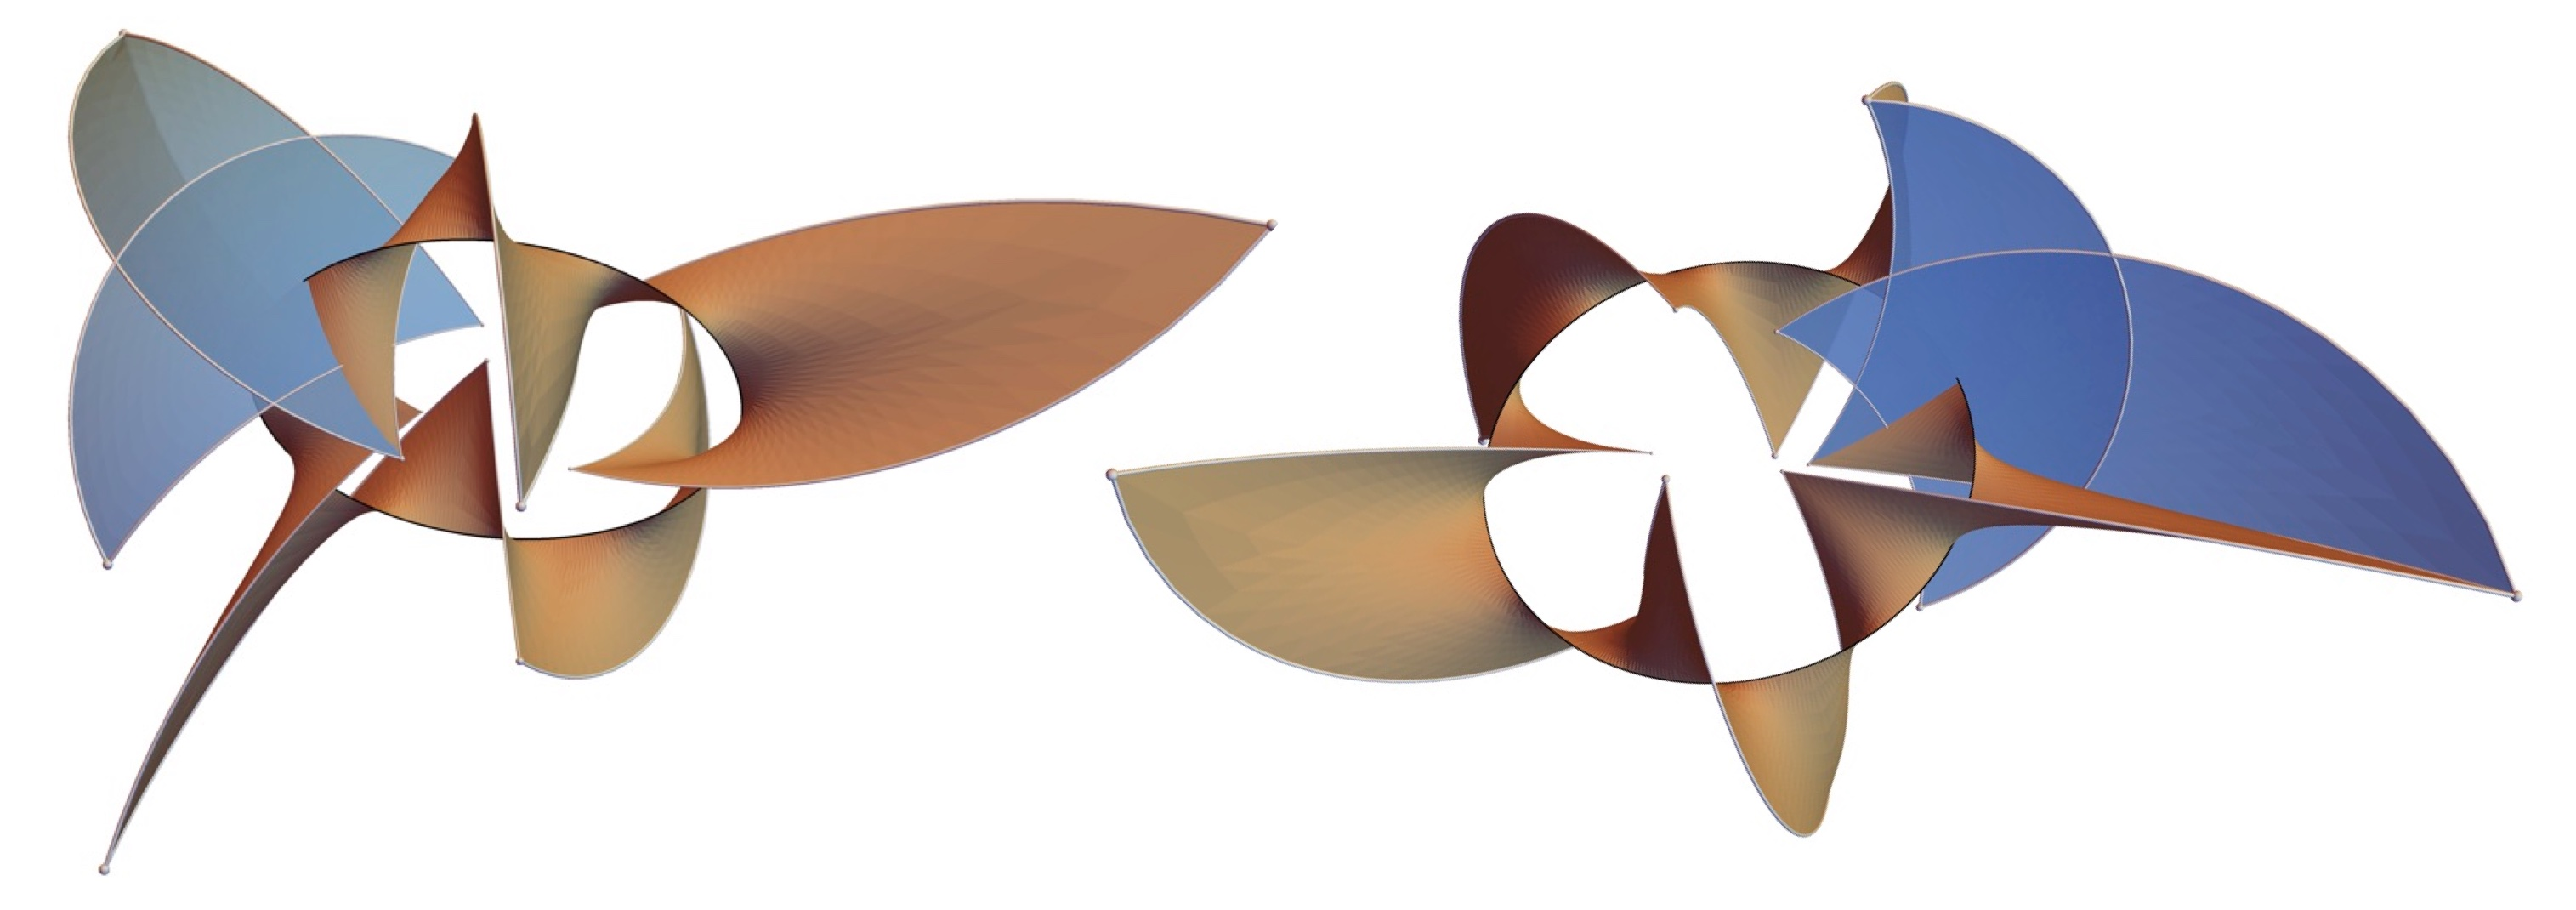
\includegraphics[width=0.95\linewidth]{2-Caras-Picudo-D.jpg}
			\caption{Stereographic projections of a face of  $\left\{\frac{12}{1,5},3,5\right\}$ depicted as a ribbon from the cycle in the 1-skeleton to the axis of its rotation, which is in $\mathbb{R}^3\cap\mathbb{S}^3$, with the base face of $\left\{\frac{5}{2},3,5\right\}$}\label{fig:12}
	\end{center}
\end{figure}
	
	We now show this structure satisfies \textit{(i)-(iv)} in our definition of skeletal 4-polytope. By the realization being faithful and symmetric, conditions \textit{(i)} and \textit{(ii)} follow from (P4) and (P3), respectively. For \textit{(iii)} notice the vertex figures are icosahedra, which follows from Wythoff's construction on any vertex adjacent to the base vertex by the group $\langle S_2,S_3\rangle$. Finally, \textit{(iv)} is immediate from the finiteness of the group. This concludes the proof that we have constructed a chiral 4-polytope.
	
%	We may also show \textit{(i)} in a slightly more geometric way. It has been shown in  \texttt{geometric.txt} that for the base face $f$,
%	\begin{equation*}\label{ec:stab-face}
%		\Stab_{\langle S_1,S_2,S_3\rangle}(f)=\langle S_1,S_2S_3\rangle,
%	\end{equation*}
%	which implies that every face belongs to exactly two cells. In fact, since $S_1$ fixes the base cell and $S_2S_3$ an involution, if any cell has $f$ as a face, we may map it to the base cell by a transformation fixing $f$.
	
	Further, it was found that there exists no automorphism $\rho$ of the group generated by the $S_i$ that satisfies \cref{eq:combinatorially-chiral}, so that the abstract polytope associated to $\left\{\frac{12}{1,5},3,5\right\}$ is combinatorially chiral (see \Cref{app:1}).
	
	
	\section{A chiral 4-polytope from $\left\{5,3,\frac{5}{2}\right\}$}
	For the dual star polytope $\left\{5,3,\frac{5}{2}\right\}$ we simply define
	\[Q_0=P_3,\qquad Q_1=P_2\qquad Q_2=P_1,\quad\text{and}\quad Q_3=P_0\]
	and apply Wythoff's construction on the centroid of the base cell of $\left\{\frac{5}{2},3,5\right\}$. This yields a realization of $\left\{5,3,\frac{5}{2}\right\}$.
	
	Analogue definitions for the $S_i$ as in the last section also satisfy \cref{eq:string-chiral} and \cref{eq:chiral-int}, so that we have another abstract 4-polytope that is, in fact, the same as the (abstract) one constructed before.
	
	Wythoff's construction on the base vertex then yields a symmetric and faithful realization of a chiral 4-polytope whose cells are copies of $H_0(\left\{5,3,\frac{5}{2}\right\})$ from \cite{petcox}. We call it $\left\{\frac{12}{1,5},3,\frac{5}{2}\right\}$.
	
\begin{figure}[H]
	
	
			\centering
			\begin{subfigure}[b]{0.5\linewidth}	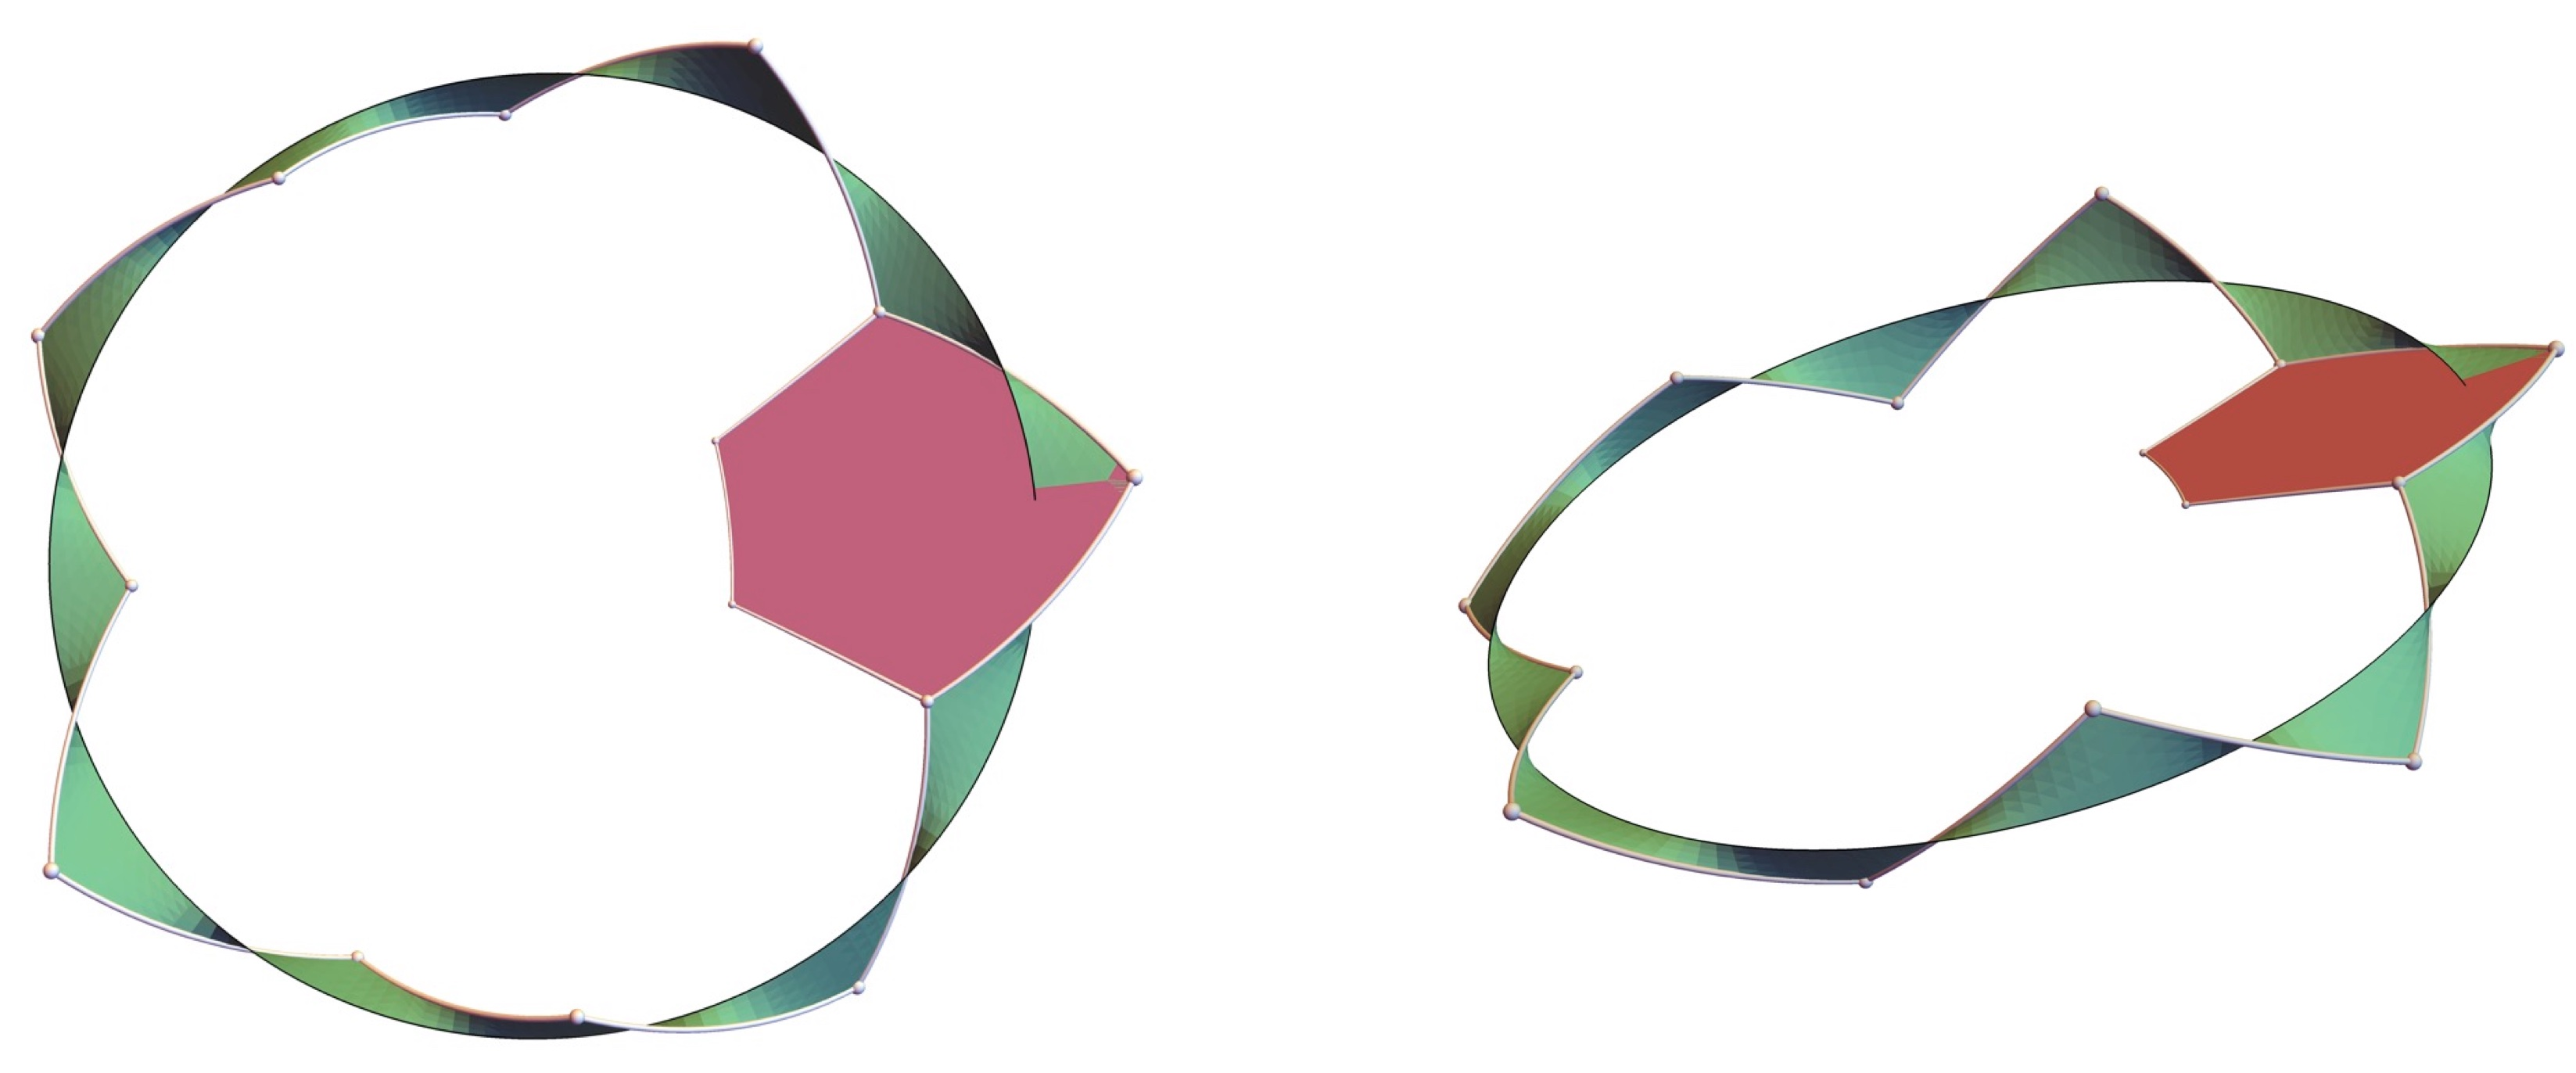
\includegraphics[width=\linewidth]{2-Caras-Plano.jpg}
			\caption{The faces of $\left\{\frac{12}{1,5},3,\frac{5}{2}\right\}$ and $\left\{5,3,\frac{5}{2}\right\}$}\label{fig:13a}
		\end{subfigure}
		\begin{subfigure}[b]{0.45\linewidth}
		\centering
        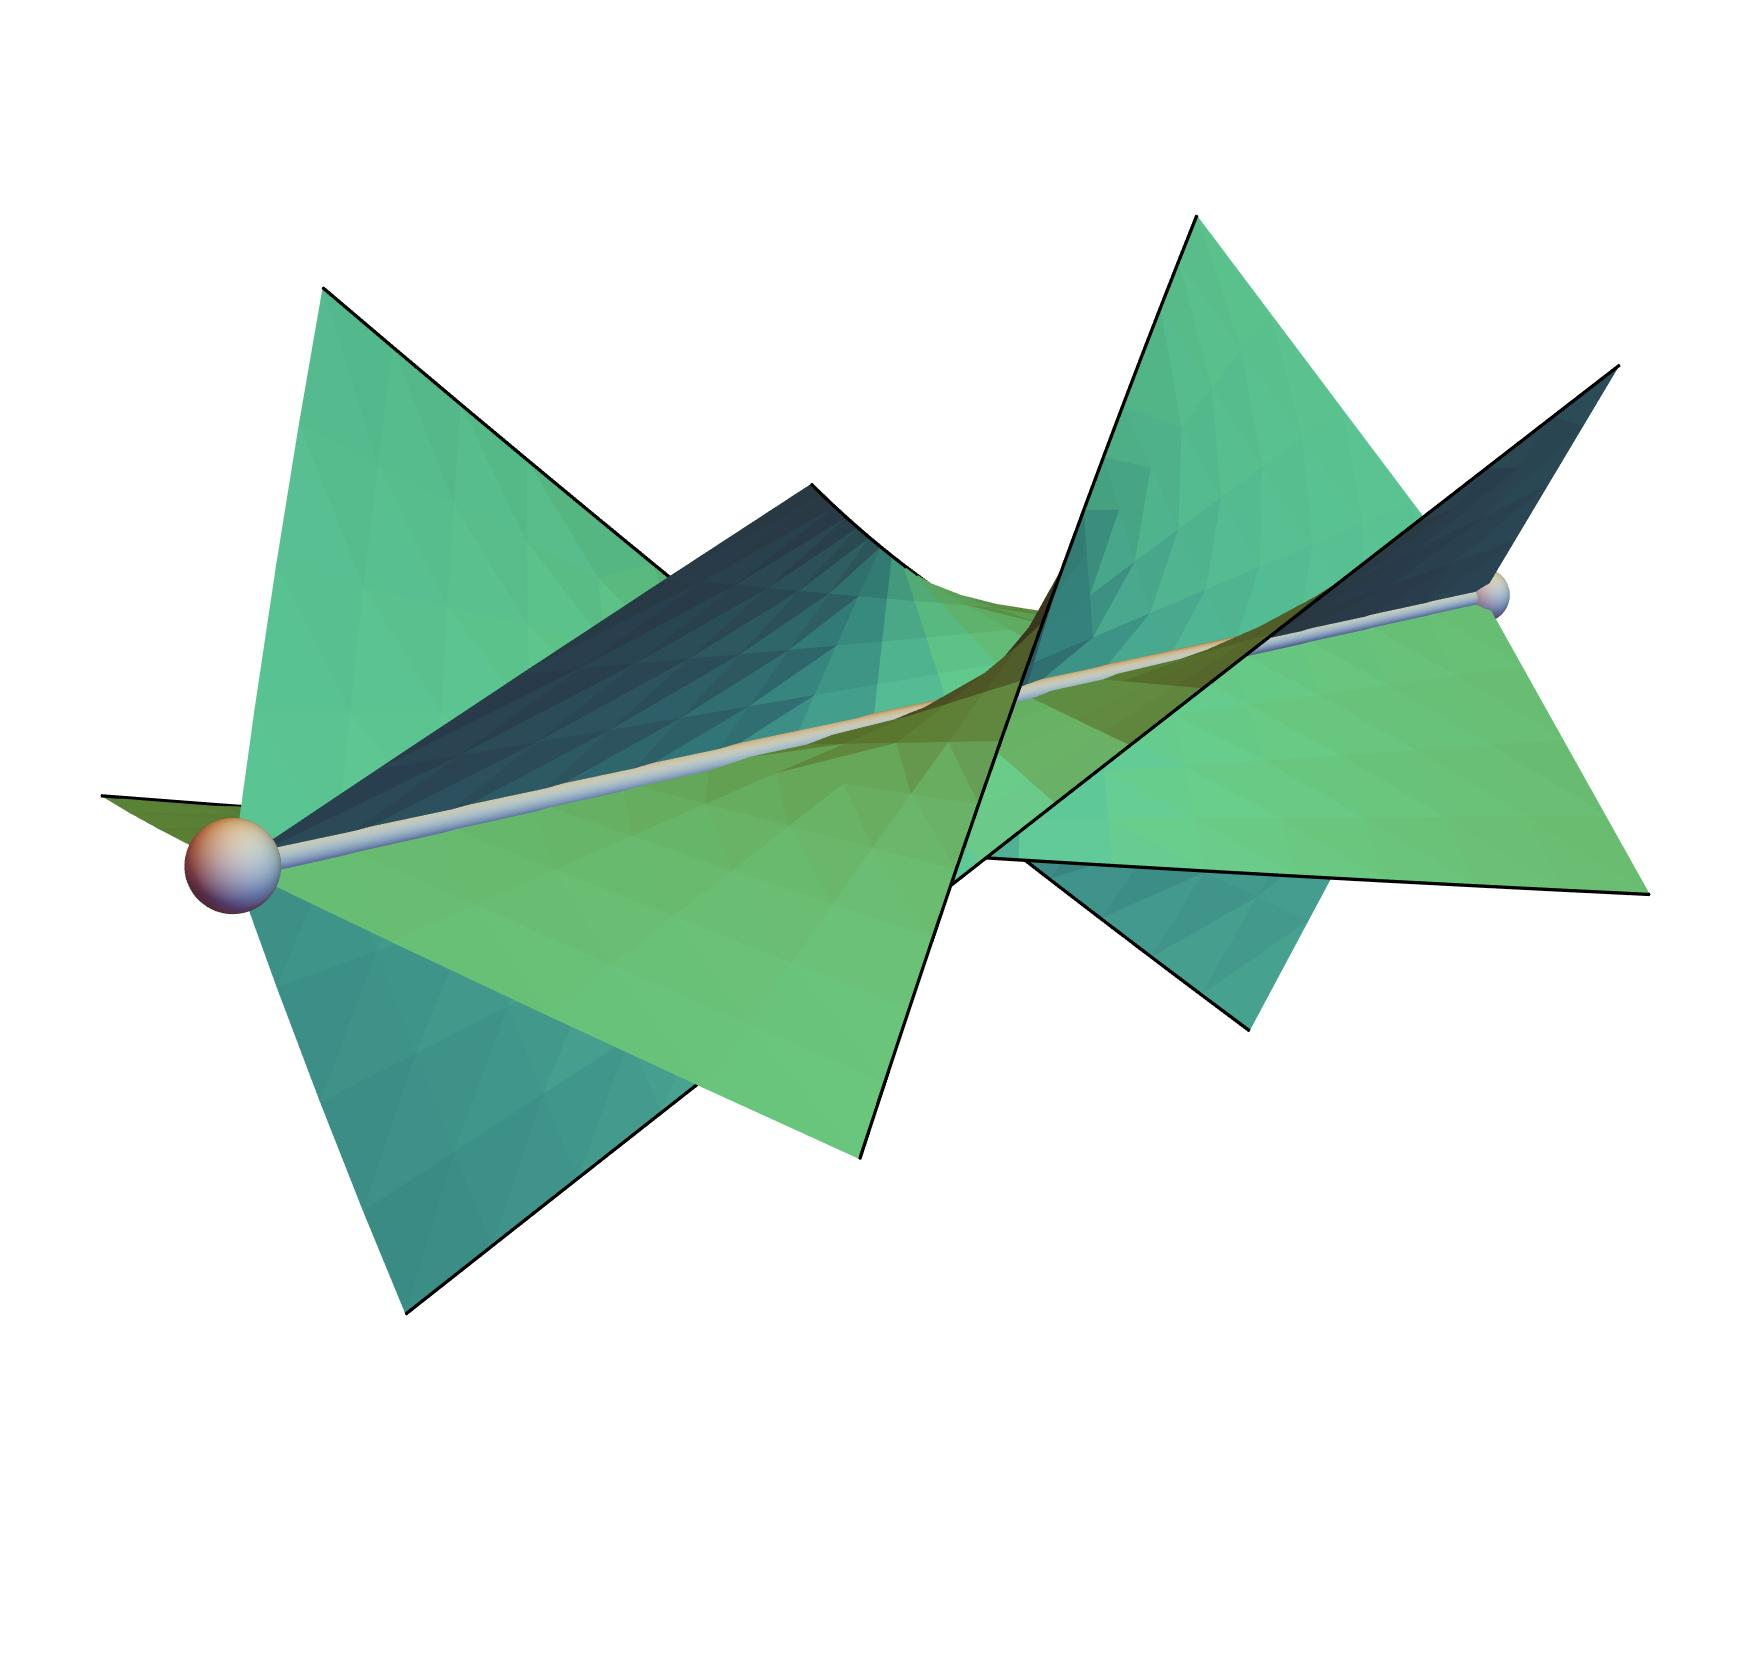
\includegraphics[width=0.6\linewidth]{Arista.jpg}
			\caption{Five faces at the edge. }\label{fig:13b}
		\end{subfigure}
	
	\caption{Stereographic projections of parts of $\left\{\frac{12}{1,5},3,\frac{5}{2}\right\}$; its faces are shown as the surface spanned between the edges and the axis of the generating twist.}\label{fig:13}
\end{figure}

%\bibliographystyle{acm} 
%\bibliography{biblio}

\printbibliography

%\bibliographystyle{plain}
%\bibliography{biblio}
\end{document}
